% Options for packages loaded elsewhere
\PassOptionsToPackage{unicode}{hyperref}
\PassOptionsToPackage{hyphens}{url}
%
\documentclass[
]{article}
\usepackage{amsmath,amssymb}
\usepackage{iftex}
\ifPDFTeX
  \usepackage[T1]{fontenc}
  \usepackage[utf8]{inputenc}
  \usepackage{textcomp} % provide euro and other symbols
\else % if luatex or xetex
  \usepackage{unicode-math} % this also loads fontspec
  \defaultfontfeatures{Scale=MatchLowercase}
  \defaultfontfeatures[\rmfamily]{Ligatures=TeX,Scale=1}
\fi
\usepackage{lmodern}
\ifPDFTeX\else
  % xetex/luatex font selection
\fi
% Use upquote if available, for straight quotes in verbatim environments
\IfFileExists{upquote.sty}{\usepackage{upquote}}{}
\IfFileExists{microtype.sty}{% use microtype if available
  \usepackage[]{microtype}
  \UseMicrotypeSet[protrusion]{basicmath} % disable protrusion for tt fonts
}{}
\makeatletter
\@ifundefined{KOMAClassName}{% if non-KOMA class
  \IfFileExists{parskip.sty}{%
    \usepackage{parskip}
  }{% else
    \setlength{\parindent}{0pt}
    \setlength{\parskip}{6pt plus 2pt minus 1pt}}
}{% if KOMA class
  \KOMAoptions{parskip=half}}
\makeatother
\usepackage{xcolor}
\usepackage[margin=1in]{geometry}
\usepackage{color}
\usepackage{fancyvrb}
\newcommand{\VerbBar}{|}
\newcommand{\VERB}{\Verb[commandchars=\\\{\}]}
\DefineVerbatimEnvironment{Highlighting}{Verbatim}{commandchars=\\\{\}}
% Add ',fontsize=\small' for more characters per line
\usepackage{framed}
\definecolor{shadecolor}{RGB}{248,248,248}
\newenvironment{Shaded}{\begin{snugshade}}{\end{snugshade}}
\newcommand{\AlertTok}[1]{\textcolor[rgb]{0.94,0.16,0.16}{#1}}
\newcommand{\AnnotationTok}[1]{\textcolor[rgb]{0.56,0.35,0.01}{\textbf{\textit{#1}}}}
\newcommand{\AttributeTok}[1]{\textcolor[rgb]{0.13,0.29,0.53}{#1}}
\newcommand{\BaseNTok}[1]{\textcolor[rgb]{0.00,0.00,0.81}{#1}}
\newcommand{\BuiltInTok}[1]{#1}
\newcommand{\CharTok}[1]{\textcolor[rgb]{0.31,0.60,0.02}{#1}}
\newcommand{\CommentTok}[1]{\textcolor[rgb]{0.56,0.35,0.01}{\textit{#1}}}
\newcommand{\CommentVarTok}[1]{\textcolor[rgb]{0.56,0.35,0.01}{\textbf{\textit{#1}}}}
\newcommand{\ConstantTok}[1]{\textcolor[rgb]{0.56,0.35,0.01}{#1}}
\newcommand{\ControlFlowTok}[1]{\textcolor[rgb]{0.13,0.29,0.53}{\textbf{#1}}}
\newcommand{\DataTypeTok}[1]{\textcolor[rgb]{0.13,0.29,0.53}{#1}}
\newcommand{\DecValTok}[1]{\textcolor[rgb]{0.00,0.00,0.81}{#1}}
\newcommand{\DocumentationTok}[1]{\textcolor[rgb]{0.56,0.35,0.01}{\textbf{\textit{#1}}}}
\newcommand{\ErrorTok}[1]{\textcolor[rgb]{0.64,0.00,0.00}{\textbf{#1}}}
\newcommand{\ExtensionTok}[1]{#1}
\newcommand{\FloatTok}[1]{\textcolor[rgb]{0.00,0.00,0.81}{#1}}
\newcommand{\FunctionTok}[1]{\textcolor[rgb]{0.13,0.29,0.53}{\textbf{#1}}}
\newcommand{\ImportTok}[1]{#1}
\newcommand{\InformationTok}[1]{\textcolor[rgb]{0.56,0.35,0.01}{\textbf{\textit{#1}}}}
\newcommand{\KeywordTok}[1]{\textcolor[rgb]{0.13,0.29,0.53}{\textbf{#1}}}
\newcommand{\NormalTok}[1]{#1}
\newcommand{\OperatorTok}[1]{\textcolor[rgb]{0.81,0.36,0.00}{\textbf{#1}}}
\newcommand{\OtherTok}[1]{\textcolor[rgb]{0.56,0.35,0.01}{#1}}
\newcommand{\PreprocessorTok}[1]{\textcolor[rgb]{0.56,0.35,0.01}{\textit{#1}}}
\newcommand{\RegionMarkerTok}[1]{#1}
\newcommand{\SpecialCharTok}[1]{\textcolor[rgb]{0.81,0.36,0.00}{\textbf{#1}}}
\newcommand{\SpecialStringTok}[1]{\textcolor[rgb]{0.31,0.60,0.02}{#1}}
\newcommand{\StringTok}[1]{\textcolor[rgb]{0.31,0.60,0.02}{#1}}
\newcommand{\VariableTok}[1]{\textcolor[rgb]{0.00,0.00,0.00}{#1}}
\newcommand{\VerbatimStringTok}[1]{\textcolor[rgb]{0.31,0.60,0.02}{#1}}
\newcommand{\WarningTok}[1]{\textcolor[rgb]{0.56,0.35,0.01}{\textbf{\textit{#1}}}}
\usepackage{graphicx}
\makeatletter
\def\maxwidth{\ifdim\Gin@nat@width>\linewidth\linewidth\else\Gin@nat@width\fi}
\def\maxheight{\ifdim\Gin@nat@height>\textheight\textheight\else\Gin@nat@height\fi}
\makeatother
% Scale images if necessary, so that they will not overflow the page
% margins by default, and it is still possible to overwrite the defaults
% using explicit options in \includegraphics[width, height, ...]{}
\setkeys{Gin}{width=\maxwidth,height=\maxheight,keepaspectratio}
% Set default figure placement to htbp
\makeatletter
\def\fps@figure{htbp}
\makeatother
\setlength{\emergencystretch}{3em} % prevent overfull lines
\providecommand{\tightlist}{%
  \setlength{\itemsep}{0pt}\setlength{\parskip}{0pt}}
\setcounter{secnumdepth}{-\maxdimen} % remove section numbering
\usepackage[labelfont={bf}]{caption}
\usepackage[unicode=true, breaklinks=true]{hyperref}
\usepackage{lmodern}
\usepackage{booktabs}
\usepackage{caption}
\usepackage{longtable}
\usepackage{colortbl}
\usepackage{array}
\ifLuaTeX
  \usepackage{selnolig}  % disable illegal ligatures
\fi
\IfFileExists{bookmark.sty}{\usepackage{bookmark}}{\usepackage{hyperref}}
\IfFileExists{xurl.sty}{\usepackage{xurl}}{} % add URL line breaks if available
\urlstyle{same}
\hypersetup{
  pdftitle={Project 2},
  pdfauthor={Suman Paudel},
  hidelinks,
  pdfcreator={LaTeX via pandoc}}

\title{Project 2}
\author{Suman Paudel}
\date{2024-03-25}

\begin{document}
\maketitle

\hypertarget{load-all-of-the-necessary-packages-need-for-this-project.}{%
\paragraph{\texorpdfstring{\textbf{Load all of the necessary packages
need for this
project.}}{Load all of the necessary packages need for this project.}}\label{load-all-of-the-necessary-packages-need-for-this-project.}}

\begin{Shaded}
\begin{Highlighting}[]
\CommentTok{\# Load the packages}
\FunctionTok{library}\NormalTok{(pdftools)}
\FunctionTok{library}\NormalTok{(tm)}
\FunctionTok{library}\NormalTok{(magrittr)}
\FunctionTok{library}\NormalTok{(wordcloud)}
\FunctionTok{library}\NormalTok{(Rgraphviz)}
\FunctionTok{library}\NormalTok{(graph)}
\FunctionTok{library}\NormalTok{(foreign) }
\FunctionTok{library}\NormalTok{(gt)}
\FunctionTok{library}\NormalTok{(tidyverse)}
\FunctionTok{library}\NormalTok{(jsonlite)}
\FunctionTok{library}\NormalTok{(httr)}
\end{Highlighting}
\end{Shaded}

\hypertarget{task-1}{%
\paragraph{\texorpdfstring{\textbf{Task 1}}{Task 1}}\label{task-1}}

Part 1

\begin{Shaded}
\begin{Highlighting}[]
\CommentTok{\# load the data using Base R read.csv }
\NormalTok{data }\OtherTok{\textless{}{-}} \FunctionTok{read.csv}\NormalTok{(}\StringTok{"covnep\_252days.csv"}\NormalTok{)}

\FunctionTok{summary}\NormalTok{(data}\SpecialCharTok{$}\NormalTok{totalCases)}
\end{Highlighting}
\end{Shaded}

\begin{verbatim}
##    Min. 1st Qu.  Median    Mean 3rd Qu.    Max. 
##       0       2     963   13376   19341   77816
\end{verbatim}

\begin{Shaded}
\begin{Highlighting}[]
\CommentTok{\# minimum value is 0 but we need 1 instead}
\CommentTok{\# this can be achieved using multiple ways like ifelse or pmax or subsetting}

\CommentTok{\# using ifelse}
\NormalTok{totalCases\_ifelse }\OtherTok{\textless{}{-}} \FunctionTok{ifelse}\NormalTok{(data}\SpecialCharTok{$}\NormalTok{totalCases }\SpecialCharTok{\textless{}} \DecValTok{1}\NormalTok{, }\DecValTok{1}\NormalTok{, data}\SpecialCharTok{$}\NormalTok{totalCases)}
\FunctionTok{summary}\NormalTok{(totalCases\_ifelse)}
\end{Highlighting}
\end{Shaded}

\begin{verbatim}
##    Min. 1st Qu.  Median    Mean 3rd Qu.    Max. 
##       1       2     963   13377   19341   77816
\end{verbatim}

\begin{Shaded}
\begin{Highlighting}[]
\CommentTok{\# using pmax}
\NormalTok{totalCases\_pmax }\OtherTok{\textless{}{-}} \FunctionTok{pmax}\NormalTok{(data}\SpecialCharTok{$}\NormalTok{totalCases, }\DecValTok{1}\NormalTok{)}
\FunctionTok{summary}\NormalTok{(totalCases\_pmax)}
\end{Highlighting}
\end{Shaded}

\begin{verbatim}
##    Min. 1st Qu.  Median    Mean 3rd Qu.    Max. 
##       1       2     963   13377   19341   77816
\end{verbatim}

\begin{Shaded}
\begin{Highlighting}[]
\CommentTok{\# subsetting}
\NormalTok{totalCases\_subsetting }\OtherTok{\textless{}{-}}\NormalTok{ data}\SpecialCharTok{$}\NormalTok{totalCases}
\NormalTok{totalCases\_subsetting[totalCases\_subsetting }\SpecialCharTok{\textless{}} \DecValTok{1}\NormalTok{] }\OtherTok{\textless{}{-}} \DecValTok{1}
\FunctionTok{summary}\NormalTok{(totalCases\_subsetting)}
\end{Highlighting}
\end{Shaded}

\begin{verbatim}
##    Min. 1st Qu.  Median    Mean 3rd Qu.    Max. 
##       1       2     963   13377   19341   77816
\end{verbatim}

Part 2

\begin{Shaded}
\begin{Highlighting}[]
\NormalTok{saq\_data }\OtherTok{\textless{}{-}} \FunctionTok{read.spss}\NormalTok{(}\StringTok{"SAQ8.sav"}\NormalTok{,}\AttributeTok{to.data.frame=}\ConstantTok{TRUE}\NormalTok{)}
\end{Highlighting}
\end{Shaded}

For q01

\begin{Shaded}
\begin{Highlighting}[]
\FunctionTok{library}\NormalTok{(foreign) }\CommentTok{\# for .SAV file we can use foreign package for that as well}
\FunctionTok{library}\NormalTok{(gt, }\AttributeTok{warn.conflicts =} \ConstantTok{FALSE}\NormalTok{) }\CommentTok{\#genotype table}
\FunctionTok{library}\NormalTok{(magrittr) }\CommentTok{\# for using pipes}
\FunctionTok{library}\NormalTok{(tibble)}
\FunctionTok{library}\NormalTok{(dplyr)}

\CommentTok{\# read the .sav file using read\_sav function from haven}
\NormalTok{saq\_data }\OtherTok{\textless{}{-}} \FunctionTok{read.spss}\NormalTok{(}\StringTok{"SAQ8.sav"}\NormalTok{,}\AttributeTok{to.data.frame=}\ConstantTok{TRUE}\NormalTok{)}


\CommentTok{\# for q1}

\NormalTok{q01 }\OtherTok{\textless{}{-}}\NormalTok{ saq\_data}\SpecialCharTok{$}\NormalTok{q01}

\NormalTok{datalevels\_q01 }\OtherTok{\textless{}{-}} \FunctionTok{levels}\NormalTok{(q01)}
\NormalTok{freq\_q01 }\OtherTok{\textless{}{-}} \FunctionTok{as.numeric}\NormalTok{(}\FunctionTok{table}\NormalTok{(q01))}
\NormalTok{percent\_q01 }\OtherTok{\textless{}{-}} \FunctionTok{as.numeric}\NormalTok{(}\FunctionTok{round}\NormalTok{(}\FunctionTok{prop.table}\NormalTok{(freq\_q01) }\SpecialCharTok{*} \DecValTok{100}\NormalTok{, }\DecValTok{1}\NormalTok{))}
\NormalTok{valid\_percent\_q01 }\OtherTok{\textless{}{-}} \FunctionTok{as.numeric}\NormalTok{(}\FunctionTok{round}\NormalTok{(}\FunctionTok{prop.table}\NormalTok{(freq\_q01) }\SpecialCharTok{*} \DecValTok{100}\NormalTok{, }\DecValTok{1}\NormalTok{))}
\NormalTok{cum\_percent }\OtherTok{\textless{}{-}} \FunctionTok{cumsum}\NormalTok{(percent\_q01)}

\CommentTok{\# Create data frame}
\NormalTok{data }\OtherTok{\textless{}{-}} \FunctionTok{data.frame}\NormalTok{(}
  \AttributeTok{Levels =}\NormalTok{ datalevels\_q01,}
  \AttributeTok{Freq =}\NormalTok{ freq\_q01,}
  \AttributeTok{Percent =}\NormalTok{ percent\_q01,}
  \AttributeTok{Val\_Percent =}\NormalTok{ valid\_percent\_q01,}
  \AttributeTok{Cum\_Percent =}\NormalTok{ cum\_percent}
\NormalTok{)}

\CommentTok{\# final version of calculated table}
\NormalTok{data }\OtherTok{\textless{}{-}}\NormalTok{ data }\SpecialCharTok{\%\textgreater{}\%} \FunctionTok{add\_row}\NormalTok{(}\AttributeTok{Levels =} \StringTok{"Total"}\NormalTok{, }\AttributeTok{Freq =} \FunctionTok{sum}\NormalTok{(data}\SpecialCharTok{$}\NormalTok{Freq), }
                 \AttributeTok{Percent =} \FunctionTok{sum}\NormalTok{(data}\SpecialCharTok{$}\NormalTok{Percent), }
                 \AttributeTok{Val\_Percent =} \FunctionTok{sum}\NormalTok{(data}\SpecialCharTok{$}\NormalTok{Val\_Percent),}
                 \AttributeTok{Cum\_Percent =} \ConstantTok{NULL}\NormalTok{)}

\CommentTok{\# aethetics table using gt}
\NormalTok{data }\SpecialCharTok{\%\textgreater{}\%} \FunctionTok{gt}\NormalTok{(}\AttributeTok{rowname\_col =} \StringTok{\textquotesingle{}Levels\textquotesingle{}}\NormalTok{) }\SpecialCharTok{\%\textgreater{}\%} 
  \FunctionTok{tab\_header}\NormalTok{(}\AttributeTok{title =} \FunctionTok{md}\NormalTok{(}\StringTok{"Statistics makes me cry"}\NormalTok{)) }\SpecialCharTok{\%\textgreater{}\%} 
  \FunctionTok{cols\_label}\NormalTok{(}\AttributeTok{Freq =} \StringTok{"Frequency"}\NormalTok{,}
             \AttributeTok{Percent =} \StringTok{"Percent"}\NormalTok{,}
             \AttributeTok{Val\_Percent =} \StringTok{"Valid Percent"}\NormalTok{,}
             \AttributeTok{Cum\_Percent =} \StringTok{"Cumulative Percent"}\NormalTok{) }\SpecialCharTok{\%\textgreater{}\%} 
  \FunctionTok{sub\_missing}\NormalTok{(}\AttributeTok{missing\_text =} \StringTok{""}\NormalTok{)}
\end{Highlighting}
\end{Shaded}

\begin{longtable}{l|rrrr}
\caption*{
{\large Statistics makes me cry}
} \\ 
\toprule
\multicolumn{1}{l}{} & Frequency & Percent & Valid Percent & Cumulative Percent \\ 
\midrule\addlinespace[2.5pt]
Strongly agree & 270 & 10.5 & 10.5 & 10.5 \\ 
Agree & 1338 & 52.0 & 52.0 & 62.5 \\ 
Neither & 735 & 28.6 & 28.6 & 91.1 \\ 
Disagree & 187 & 7.3 & 7.3 & 98.4 \\ 
Strongly disagree & 41 & 1.6 & 1.6 & 100.0 \\ 
Total & 2571 & 100.0 & 100.0 &  \\ 
\bottomrule
\end{longtable}

\begin{Shaded}
\begin{Highlighting}[]
\CommentTok{\# for q03}

\NormalTok{q03 }\OtherTok{\textless{}{-}}\NormalTok{ saq\_data}\SpecialCharTok{$}\NormalTok{q03}
\NormalTok{datalevels\_q03 }\OtherTok{\textless{}{-}} \FunctionTok{levels}\NormalTok{(q03)}
\NormalTok{freq\_q03 }\OtherTok{\textless{}{-}} \FunctionTok{as.numeric}\NormalTok{(}\FunctionTok{table}\NormalTok{(q03))}
\NormalTok{percent\_q03 }\OtherTok{\textless{}{-}} \FunctionTok{as.numeric}\NormalTok{(}\FunctionTok{round}\NormalTok{(}\FunctionTok{prop.table}\NormalTok{(freq\_q03) }\SpecialCharTok{*} \DecValTok{100}\NormalTok{, }\DecValTok{1}\NormalTok{))}
\NormalTok{valid\_percent\_q03 }\OtherTok{\textless{}{-}} \FunctionTok{as.numeric}\NormalTok{(}\FunctionTok{round}\NormalTok{(}\FunctionTok{prop.table}\NormalTok{(freq\_q03) }\SpecialCharTok{*} \DecValTok{100}\NormalTok{, }\DecValTok{1}\NormalTok{))}
\NormalTok{cum\_percent\_q03 }\OtherTok{\textless{}{-}} \FunctionTok{cumsum}\NormalTok{(percent\_q03)}

\NormalTok{data\_q03 }\OtherTok{\textless{}{-}} \FunctionTok{data.frame}\NormalTok{(}
  \AttributeTok{Levels =}\NormalTok{ datalevels\_q03,}
  \AttributeTok{Freq =}\NormalTok{ freq\_q03,}
  \AttributeTok{Percent =}\NormalTok{ percent\_q03,}
  \AttributeTok{Val\_Percent =}\NormalTok{ valid\_percent\_q03,}
  \AttributeTok{Cum\_Percent =}\NormalTok{ cum\_percent\_q03}
\NormalTok{)}

\NormalTok{data\_q03 }\OtherTok{\textless{}{-}}\NormalTok{ data\_q03 }\SpecialCharTok{\%\textgreater{}\%} \FunctionTok{add\_row}\NormalTok{(}\AttributeTok{Levels =} \StringTok{"Total"}\NormalTok{, }\AttributeTok{Freq =} \FunctionTok{sum}\NormalTok{(data\_q03}\SpecialCharTok{$}\NormalTok{Freq), }
                         \AttributeTok{Percent =} \FunctionTok{sum}\NormalTok{(data\_q03}\SpecialCharTok{$}\NormalTok{Percent), }
                         \AttributeTok{Val\_Percent =} \FunctionTok{sum}\NormalTok{(data\_q03}\SpecialCharTok{$}\NormalTok{Val\_Percent),}
                         \AttributeTok{Cum\_Percent =} \ConstantTok{NULL}\NormalTok{)}

\CommentTok{\# final version of calculated table}
\NormalTok{data\_q03 }\SpecialCharTok{\%\textgreater{}\%} \FunctionTok{gt}\NormalTok{(}\AttributeTok{rowname\_col =} \StringTok{\textquotesingle{}Levels\textquotesingle{}}\NormalTok{) }\SpecialCharTok{\%\textgreater{}\%} 
  \FunctionTok{tab\_header}\NormalTok{(}\AttributeTok{title =} \FunctionTok{md}\NormalTok{(}\StringTok{"Statistic makes me cry"}\NormalTok{)) }\SpecialCharTok{\%\textgreater{}\%} 
  \FunctionTok{cols\_label}\NormalTok{(}\AttributeTok{Freq =} \StringTok{"Frequency"}\NormalTok{,}
             \AttributeTok{Percent =} \StringTok{"Percent"}\NormalTok{,}
             \AttributeTok{Val\_Percent =} \StringTok{"Valid Percent"}\NormalTok{,}
             \AttributeTok{Cum\_Percent =} \StringTok{"Cumulative Percent"}\NormalTok{) }\SpecialCharTok{\%\textgreater{}\%} 
  \FunctionTok{sub\_missing}\NormalTok{(}\AttributeTok{missing\_text =} \StringTok{""}\NormalTok{)}
\end{Highlighting}
\end{Shaded}

\begin{longtable}{l|rrrr}
\caption*{
{\large Statistic makes me cry}
} \\ 
\toprule
\multicolumn{1}{l}{} & Frequency & Percent & Valid Percent & Cumulative Percent \\ 
\midrule\addlinespace[2.5pt]
Strongly agree & 497 & 19.3 & 19.3 & 19.3 \\ 
Agree & 672 & 26.1 & 26.1 & 45.4 \\ 
Neither & 878 & 34.2 & 34.2 & 79.6 \\ 
Disagree & 448 & 17.4 & 17.4 & 97.0 \\ 
Strongly disagree & 76 & 3.0 & 3.0 & 100.0 \\ 
Total & 2571 & 100.0 & 100.0 &  \\ 
\bottomrule
\end{longtable}

\begin{Shaded}
\begin{Highlighting}[]
\NormalTok{q06 }\OtherTok{\textless{}{-}}\NormalTok{ saq\_data}\SpecialCharTok{$}\NormalTok{q06}

\NormalTok{datalevels\_q06 }\OtherTok{\textless{}{-}} \FunctionTok{levels}\NormalTok{(q06)}
\NormalTok{freq\_q06 }\OtherTok{\textless{}{-}} \FunctionTok{as.numeric}\NormalTok{(}\FunctionTok{table}\NormalTok{(q06))}
\NormalTok{percent\_q06 }\OtherTok{\textless{}{-}} \FunctionTok{as.numeric}\NormalTok{(}\FunctionTok{round}\NormalTok{(}\FunctionTok{prop.table}\NormalTok{(freq\_q06) }\SpecialCharTok{*} \DecValTok{100}\NormalTok{, }\DecValTok{1}\NormalTok{))}
\NormalTok{valid\_percent\_q06 }\OtherTok{\textless{}{-}} \FunctionTok{as.numeric}\NormalTok{(}\FunctionTok{round}\NormalTok{(}\FunctionTok{prop.table}\NormalTok{(freq\_q06) }\SpecialCharTok{*} \DecValTok{100}\NormalTok{, }\DecValTok{1}\NormalTok{))}
\NormalTok{cum\_percent\_q06 }\OtherTok{\textless{}{-}} \FunctionTok{cumsum}\NormalTok{(percent\_q06)}

\NormalTok{data\_q06 }\OtherTok{\textless{}{-}} \FunctionTok{data.frame}\NormalTok{(}
  \AttributeTok{Levels =}\NormalTok{ datalevels\_q06,}
  \AttributeTok{Freq =}\NormalTok{ freq\_q06,}
  \AttributeTok{Percent =}\NormalTok{ percent\_q06,}
  \AttributeTok{Val\_Percent =}\NormalTok{ valid\_percent\_q06,}
  \AttributeTok{Cum\_Percent =}\NormalTok{ cum\_percent\_q06}
\NormalTok{)}

\NormalTok{data\_q06 }\OtherTok{\textless{}{-}}\NormalTok{ data\_q06 }\SpecialCharTok{\%\textgreater{}\%} \FunctionTok{add\_row}\NormalTok{(}\AttributeTok{Levels =} \StringTok{"Total"}\NormalTok{, }\AttributeTok{Freq =} \FunctionTok{sum}\NormalTok{(data\_q06}\SpecialCharTok{$}\NormalTok{Freq), }
                         \AttributeTok{Percent =} \FunctionTok{sum}\NormalTok{(data\_q06}\SpecialCharTok{$}\NormalTok{Percent), }
                         \AttributeTok{Val\_Percent =} \FunctionTok{sum}\NormalTok{(data\_q06}\SpecialCharTok{$}\NormalTok{Val\_Percent),}
                         \AttributeTok{Cum\_Percent =} \ConstantTok{NULL}\NormalTok{)}

\CommentTok{\# final version of calculated table}
\NormalTok{data\_q06 }\SpecialCharTok{\%\textgreater{}\%} \FunctionTok{gt}\NormalTok{(}\AttributeTok{rowname\_col =} \StringTok{\textquotesingle{}Levels\textquotesingle{}}\NormalTok{) }\SpecialCharTok{\%\textgreater{}\%} 
  \FunctionTok{tab\_header}\NormalTok{(}\AttributeTok{title =} \FunctionTok{md}\NormalTok{(}\StringTok{"I have little experience of computer"}\NormalTok{)) }\SpecialCharTok{\%\textgreater{}\%} 
  \FunctionTok{cols\_label}\NormalTok{(}\AttributeTok{Freq =} \StringTok{"Frequency"}\NormalTok{,}
             \AttributeTok{Percent =} \StringTok{"Percent"}\NormalTok{,}
             \AttributeTok{Val\_Percent =} \StringTok{"Valid Percent"}\NormalTok{,}
             \AttributeTok{Cum\_Percent =} \StringTok{"Cumulative Percent"}\NormalTok{) }\SpecialCharTok{\%\textgreater{}\%} 
  \FunctionTok{sub\_missing}\NormalTok{(}\AttributeTok{missing\_text =} \StringTok{""}\NormalTok{)}
\end{Highlighting}
\end{Shaded}

\begin{longtable}{l|rrrr}
\caption*{
{\large I have little experience of computer}
} \\ 
\toprule
\multicolumn{1}{l}{} & Frequency & Percent & Valid Percent & Cumulative Percent \\ 
\midrule\addlinespace[2.5pt]
Strongly agree & 702 & 27.3 & 27.3 & 27.3 \\ 
Agree & 1127 & 43.8 & 43.8 & 71.1 \\ 
Neither & 344 & 13.4 & 13.4 & 84.5 \\ 
Disagree & 252 & 9.8 & 9.8 & 94.3 \\ 
Strongly disagree & 146 & 5.7 & 5.7 & 100.0 \\ 
Total & 2571 & 100.0 & 100.0 &  \\ 
\bottomrule
\end{longtable}

\begin{Shaded}
\begin{Highlighting}[]
\NormalTok{q08 }\OtherTok{\textless{}{-}}\NormalTok{ saq\_data}\SpecialCharTok{$}\NormalTok{q08}

\NormalTok{datalevels\_q08 }\OtherTok{\textless{}{-}} \FunctionTok{levels}\NormalTok{(q08)}
\NormalTok{freq\_q08 }\OtherTok{\textless{}{-}} \FunctionTok{as.numeric}\NormalTok{(}\FunctionTok{table}\NormalTok{(q08))}
\NormalTok{percent\_q08 }\OtherTok{\textless{}{-}} \FunctionTok{as.numeric}\NormalTok{(}\FunctionTok{round}\NormalTok{(}\FunctionTok{prop.table}\NormalTok{(freq\_q08) }\SpecialCharTok{*} \DecValTok{100}\NormalTok{, }\DecValTok{2}\NormalTok{))}
\NormalTok{valid\_percent\_q08 }\OtherTok{\textless{}{-}} \FunctionTok{as.numeric}\NormalTok{(}\FunctionTok{round}\NormalTok{(}\FunctionTok{prop.table}\NormalTok{(freq\_q08) }\SpecialCharTok{*} \DecValTok{100}\NormalTok{, }\DecValTok{2}\NormalTok{))}
\NormalTok{cum\_percent\_q08 }\OtherTok{\textless{}{-}} \FunctionTok{cumsum}\NormalTok{(percent\_q08)}


\NormalTok{data\_q08 }\OtherTok{\textless{}{-}} \FunctionTok{data.frame}\NormalTok{(}
  \AttributeTok{Levels =}\NormalTok{ datalevels\_q08,}
  \AttributeTok{Freq =}\NormalTok{ freq\_q08,}
  \AttributeTok{Percent =} \FunctionTok{round}\NormalTok{(valid\_percent\_q08,}\DecValTok{1}\NormalTok{),}
  \AttributeTok{Val\_Percent =} \FunctionTok{round}\NormalTok{(valid\_percent\_q08,}\DecValTok{1}\NormalTok{),}
  \AttributeTok{Cum\_Percent =} \FunctionTok{round}\NormalTok{(cum\_percent\_q08,}\DecValTok{1}\NormalTok{)}
\NormalTok{)}

\NormalTok{data\_q08 }\OtherTok{\textless{}{-}}\NormalTok{ data\_q08 }\SpecialCharTok{\%\textgreater{}\%} \FunctionTok{add\_row}\NormalTok{(}\AttributeTok{Levels =} \StringTok{"Total"}\NormalTok{, }\AttributeTok{Freq =} \FunctionTok{sum}\NormalTok{(data\_q06}\SpecialCharTok{$}\NormalTok{Freq), }
                         \AttributeTok{Percent =} \FunctionTok{sum}\NormalTok{(data\_q08}\SpecialCharTok{$}\NormalTok{Percent), }
                         \AttributeTok{Val\_Percent =} \FunctionTok{sum}\NormalTok{(data\_q08}\SpecialCharTok{$}\NormalTok{Val\_Percent),}
                         \AttributeTok{Cum\_Percent =} \ConstantTok{NULL}\NormalTok{)}


\CommentTok{\# final version of calculated table}
\NormalTok{data\_q08 }\SpecialCharTok{\%\textgreater{}\%} \FunctionTok{gt}\NormalTok{(}\AttributeTok{rowname\_col =} \StringTok{\textquotesingle{}Levels\textquotesingle{}}\NormalTok{) }\SpecialCharTok{\%\textgreater{}\%} 
  \FunctionTok{tab\_header}\NormalTok{(}\AttributeTok{title =} \FunctionTok{md}\NormalTok{(}\StringTok{"Statistics makes me cry"}\NormalTok{)) }\SpecialCharTok{\%\textgreater{}\%} 
  \FunctionTok{cols\_label}\NormalTok{(}\AttributeTok{Freq =} \StringTok{"Frequency"}\NormalTok{,}
             \AttributeTok{Percent =} \StringTok{"Percent"}\NormalTok{,}
             \AttributeTok{Val\_Percent =} \StringTok{"Valid Percent"}\NormalTok{,}
             \AttributeTok{Cum\_Percent =} \StringTok{"Cumulative Percent"}\NormalTok{) }\SpecialCharTok{\%\textgreater{}\%} 
  \FunctionTok{sub\_missing}\NormalTok{(}\AttributeTok{missing\_text =} \StringTok{""}\NormalTok{)}
\end{Highlighting}
\end{Shaded}

\begin{longtable}{l|rrrr}
\caption*{
{\large Statistics makes me cry}
} \\ 
\toprule
\multicolumn{1}{l}{} & Frequency & Percent & Valid Percent & Cumulative Percent \\ 
\midrule\addlinespace[2.5pt]
Strongly agree & 383 & 14.9 & 14.9 & 14.9 \\ 
Agree & 1487 & 57.8 & 57.8 & 72.7 \\ 
Neither & 482 & 18.8 & 18.8 & 91.5 \\ 
Disagree & 147 & 5.7 & 5.7 & 97.2 \\ 
Strongly disagree & 72 & 2.8 & 2.8 & 100.0 \\ 
Total & 5142 & 100.0 & 100.0 &  \\ 
\bottomrule
\end{longtable}

\hypertarget{task-2-web-scraping}{%
\paragraph{\texorpdfstring{\textbf{Task 2} Web
Scraping}{Task 2 Web Scraping}}\label{task-2-web-scraping}}

\begin{Shaded}
\begin{Highlighting}[]
\NormalTok{data\_1 }\OtherTok{=} \StringTok{\textquotesingle{}https://data.covid19india.org/v4/min/timeseries.min.json\textquotesingle{}}
\NormalTok{data\_2 }\OtherTok{=} \StringTok{\textquotesingle{}https://data.covid19india.org/v4/min/data.min.json\textquotesingle{}}
\NormalTok{covid\_data\_1 }\OtherTok{\textless{}{-}}\NormalTok{ jsonlite}\SpecialCharTok{::}\FunctionTok{fromJSON}\NormalTok{(data\_1)}
\NormalTok{covid\_data\_2 }\OtherTok{\textless{}{-}}\NormalTok{ jsonlite}\SpecialCharTok{::}\FunctionTok{fromJSON}\NormalTok{(data\_2)}
\end{Highlighting}
\end{Shaded}

\begin{Shaded}
\begin{Highlighting}[]
\NormalTok{covid\_1\_parsed }\OtherTok{\textless{}{-}}
\NormalTok{  covid\_data\_1 }\SpecialCharTok{\%\textgreater{}\%} \FunctionTok{enframe}\NormalTok{() }\SpecialCharTok{\%\textgreater{}\%} \FunctionTok{unnest\_wider}\NormalTok{(value) }\SpecialCharTok{\%\textgreater{}\%} \FunctionTok{unnest\_wider}\NormalTok{(dates) }\SpecialCharTok{\%\textgreater{}\%}
  \FunctionTok{pivot\_longer}\NormalTok{(}\AttributeTok{cols =} \SpecialCharTok{!}\NormalTok{name,}
               \AttributeTok{names\_to =} \StringTok{\textquotesingle{}date\textquotesingle{}}\NormalTok{,}
               \AttributeTok{values\_to =} \StringTok{"value"}\NormalTok{) }\SpecialCharTok{\%\textgreater{}\%} \FunctionTok{unnest\_wider}\NormalTok{(value) }\SpecialCharTok{\%\textgreater{}\%}
  \FunctionTok{mutate}\NormalTok{(}\FunctionTok{across}\NormalTok{(}\FunctionTok{c}\NormalTok{(delta, delta7, total), }\SpecialCharTok{\textasciitilde{}} \FunctionTok{map}\NormalTok{(., }\SpecialCharTok{\textasciitilde{}} \FunctionTok{set\_names}\NormalTok{(}
    \FunctionTok{as\_tibble}\NormalTok{(.x), }\FunctionTok{paste0}\NormalTok{(}\FunctionTok{cur\_column}\NormalTok{(), }\StringTok{"\_"}\NormalTok{, }\FunctionTok{names}\NormalTok{(.))}
\NormalTok{  )))) }\SpecialCharTok{\%\textgreater{}\%}
  \FunctionTok{unnest\_wider}\NormalTok{(}\FunctionTok{c}\NormalTok{(delta, delta7, total))}

\NormalTok{covid\_1\_parsed[}\DecValTok{150}\SpecialCharTok{:}\DecValTok{300}\NormalTok{, }\FunctionTok{c}\NormalTok{(}\StringTok{"delta\_confirmed"}\NormalTok{,}\StringTok{"delta\_recovered"}\NormalTok{,}\StringTok{"delta\_tested"}\NormalTok{,}\StringTok{"delta7\_confirmed"}\NormalTok{,}\StringTok{"delta7\_recovered"}\NormalTok{,}\StringTok{"delta\_tested"}\NormalTok{)]}
\end{Highlighting}
\end{Shaded}

\begin{verbatim}
## # A tibble: 151 x 6
##    delta_confirmed delta_recovered delta_tested delta7_confirmed
##              <int>           <int>        <int>            <int>
##  1              61             109          315              502
##  2              52             110          390              461
##  3              44             129          235              459
##  4              41             139          569              416
##  5              40              78          564              381
##  6              33              65          184              338
##  7              32              70          270              303
##  8              31              75          307              273
##  9              23              67          267              244
## 10              28              61          811              228
## # i 141 more rows
## # i 2 more variables: delta7_recovered <int>, delta_tested <int>
\end{verbatim}

\begin{Shaded}
\begin{Highlighting}[]
\NormalTok{covid\_2\_parsed }\OtherTok{\textless{}{-}}\NormalTok{ covid\_data\_2 }\SpecialCharTok{\%\textgreater{}\%} \FunctionTok{enframe}\NormalTok{() }\SpecialCharTok{\%\textgreater{}\%} \FunctionTok{unnest\_wider}\NormalTok{(value) }\SpecialCharTok{\%\textgreater{}\%} 
  \FunctionTok{unnest\_wider}\NormalTok{(}\FunctionTok{c}\NormalTok{(delta,delta21\_14, delta7, total),}\AttributeTok{names\_sep =} \StringTok{"\_"}\NormalTok{) }\SpecialCharTok{\%\textgreater{}\%} \FunctionTok{select}\NormalTok{(}\SpecialCharTok{{-}}\FunctionTok{c}\NormalTok{(districts,meta))}
\NormalTok{covid\_2\_parsed[, }\FunctionTok{c}\NormalTok{(}\StringTok{"delta\_confirmed"}\NormalTok{,}\StringTok{"delta\_recovered"}\NormalTok{,}\StringTok{"delta\_tested"}\NormalTok{,}\StringTok{"delta7\_confirmed"}\NormalTok{,}\StringTok{"delta7\_recovered"}\NormalTok{,}\StringTok{"delta\_tested"}\NormalTok{)]}
\end{Highlighting}
\end{Shaded}

\begin{verbatim}
## # A tibble: 37 x 6
##    delta_confirmed delta_recovered delta_tested delta7_confirmed
##              <int>           <int>        <int>            <int>
##  1              NA              NA         1376                3
##  2             385             675        39848             2873
##  3               1               9          334               66
##  4             212             236        15060             2056
##  5               8               9       226443               40
##  6               5               3         1403               28
##  7              32              32        11869              205
##  8              45              46        56751              267
##  9              NA               1           NA               NA
## 10              23              53         2361              222
## # i 27 more rows
## # i 2 more variables: delta7_recovered <int>, delta_tested <int>
\end{verbatim}

\begin{Shaded}
\begin{Highlighting}[]
\NormalTok{merged\_df }\OtherTok{\textless{}{-}} \FunctionTok{merge}\NormalTok{(covid\_1\_parsed, covid\_2\_parsed, }\AttributeTok{by =} \StringTok{"name"}\NormalTok{, }\AttributeTok{all =} \ConstantTok{FALSE}\NormalTok{)}
\FunctionTok{head}\NormalTok{(merged\_df[}\DecValTok{7250}\SpecialCharTok{:}\DecValTok{8000}\NormalTok{,])}
\end{Highlighting}
\end{Shaded}

\begin{verbatim}
##      name       date delta_confirmed.x delta_recovered.x delta_tested.x
## 7250   HP 2021-04-20              1340              1078           9744
## 7251   HP 2021-04-21              1692               908           9291
## 7252   HP 2021-04-22              1774               689           8037
## 7253   HP 2021-04-23              1189               772          10385
## 7254   HP 2021-04-24              2073               877          10534
## 7255   HP 2021-04-25              1363              1161           7164
##      delta_other.x delta_deceased.x delta_vaccinated1.x delta_vaccinated2.x
## 7250            NA               16               40934                9089
## 7251            NA               17               18780                3381
## 7252             4               18               41362                9161
## 7253             4               26               36710                9874
## 7254             7               24               32168                7402
## 7255             4               32                8353                2612
##      delta7_confirmed.x delta7_recovered.x delta7_tested.x delta7_other.x
## 7250               8016               4184           54645            -12
## 7251               8783               4840           56298            -12
## 7252               9523               4940           58520             -9
## 7253               9870               5228           62516             -5
## 7254              10551               5449           62143             11
## 7255              11126               6078           60798             21
##      delta7_deceased.x delta7_vaccinated1.x delta7_vaccinated2.x
## 7250                84               228964                37855
## 7251                88               204933                37985
## 7252                95               215432                43395
## 7253               112               209999                46366
## 7254               124               211167                48268
## 7255               146               210197                48792
##      total_confirmed.x total_recovered.x total_tested.x total_other.x
## 7250             79410             68150        1401986            25
## 7251             81102             69058        1411277            25
## 7252             82876             69747        1419314            29
## 7253             84065             70519        1429699            33
## 7254             86138             71396        1440233            40
## 7255             87501             72557        1447397            44
##      total_deceased.x total_vaccinated1.x total_vaccinated2.x delta_tested.y
## 7250             1206             1225881              152805           3613
## 7251             1223             1244661              156186           3613
## 7252             1241             1286023              165347           3613
## 7253             1267             1322733              175221           3613
## 7254             1291             1354901              182623           3613
## 7255             1323             1363254              185235           3613
##      delta_vaccinated1.y delta_vaccinated2.y delta_confirmed.y delta_deceased.y
## 7250                 371                8192                85                1
## 7251                 371                8192                85                1
## 7252                 371                8192                85                1
## 7253                 371                8192                85                1
## 7254                 371                8192                85                1
## 7255                 371                8192                85                1
##      delta_recovered.y delta_other.y delta21_14_confirmed delta7_confirmed.y
## 7250               198            NA                  958               1537
## 7251               198            NA                  958               1537
## 7252               198            NA                  958               1537
## 7253               198            NA                  958               1537
## 7254               198            NA                  958               1537
## 7255               198            NA                  958               1537
##      delta7_recovered.y delta7_tested.y delta7_vaccinated1.y
## 7250               1154           64352                13244
## 7251               1154           64352                13244
## 7252               1154           64352                13244
## 7253               1154           64352                13244
## 7254               1154           64352                13244
## 7255               1154           64352                13244
##      delta7_vaccinated2.y delta7_deceased.y delta7_other.y total_confirmed.y
## 7250               234011                20             -1            224106
## 7251               234011                20             -1            224106
## 7252               234011                20             -1            224106
## 7253               234011                20             -1            224106
## 7254               234011                20             -1            224106
## 7255               234011                20             -1            224106
##      total_deceased.y total_recovered.y total_tested.y total_vaccinated1.y
## 7250             3738            218410        3685011             5713695
## 7251             3738            218410        3685011             5713695
## 7252             3738            218410        3685011             5713695
## 7253             3738            218410        3685011             5713695
## 7254             3738            218410        3685011             5713695
## 7255             3738            218410        3685011             5713695
##      total_vaccinated2.y total_other.y
## 7250             3443823            16
## 7251             3443823            16
## 7252             3443823            16
## 7253             3443823            16
## 7254             3443823            16
## 7255             3443823            16
\end{verbatim}

\begin{Shaded}
\begin{Highlighting}[]
\FunctionTok{library}\NormalTok{(RSelenium)}
\FunctionTok{library}\NormalTok{(rvest)}
\FunctionTok{library}\NormalTok{(netstat)}
\NormalTok{rD }\OtherTok{\textless{}{-}} \FunctionTok{rsDriver}\NormalTok{(}\AttributeTok{browser=}\StringTok{"firefox"}\NormalTok{,}\AttributeTok{verbose =}\NormalTok{ F, }\AttributeTok{port =}\NormalTok{ 14421L)}
\NormalTok{remDr }\OtherTok{\textless{}{-}}\NormalTok{ rD[[}\StringTok{"client"}\NormalTok{]]}
\NormalTok{remDr}\SpecialCharTok{$}\FunctionTok{navigate}\NormalTok{(}\StringTok{"https://aqicn.org/forecast/kathmandu/"}\NormalTok{)}
\NormalTok{aqi\_html  }\OtherTok{\textless{}{-}} \FunctionTok{read\_html}\NormalTok{(remDr}\SpecialCharTok{$}\FunctionTok{getPageSource}\NormalTok{() }\SpecialCharTok{\%\textgreater{}\%} \FunctionTok{unlist}\NormalTok{())}
\NormalTok{aqi\_html }\SpecialCharTok{\%\textgreater{}\%} \FunctionTok{html\_element}\NormalTok{(}\StringTok{".forecast{-}body{-}table"}\NormalTok{) }\SpecialCharTok{\%\textgreater{}\%}  \FunctionTok{html\_nodes}\NormalTok{(}\StringTok{"table"}\NormalTok{) }\SpecialCharTok{\%\textgreater{}\%} \FunctionTok{html\_table}\NormalTok{() }\OtherTok{{-}\textgreater{}}\NormalTok{ forecast\_table}



\NormalTok{aqi\_table }\OtherTok{\textless{}{-}}\NormalTok{ forecast\_table }\SpecialCharTok{\%\textgreater{}\%}\NormalTok{ .[[}\DecValTok{1}\NormalTok{]]}


\NormalTok{aqi\_table }\OtherTok{\textless{}{-}}\NormalTok{ aqi\_table }\SpecialCharTok{\%\textgreater{}\%} \FunctionTok{select}\NormalTok{(}\SpecialCharTok{{-}}\FunctionTok{c}\NormalTok{(}\StringTok{\textquotesingle{}X10\textquotesingle{}}\NormalTok{,}\StringTok{\textquotesingle{}X11\textquotesingle{}}\NormalTok{,}\StringTok{\textquotesingle{}X20\textquotesingle{}}\NormalTok{,}\StringTok{\textquotesingle{}X21\textquotesingle{}}\NormalTok{,}\StringTok{\textquotesingle{}X30\textquotesingle{}}\NormalTok{,}\StringTok{\textquotesingle{}X31\textquotesingle{}}\NormalTok{,}\StringTok{\textquotesingle{}X40\textquotesingle{}}\NormalTok{,}\StringTok{\textquotesingle{}X41\textquotesingle{}}\NormalTok{,}\StringTok{\textquotesingle{}X50\textquotesingle{}}\NormalTok{,}\StringTok{\textquotesingle{}X51\textquotesingle{}}\NormalTok{,}\StringTok{\textquotesingle{}X60\textquotesingle{}}\NormalTok{,}\StringTok{\textquotesingle{}X61\textquotesingle{}}\NormalTok{))}

\NormalTok{aqi\_table }\OtherTok{\textless{}{-}}\NormalTok{ aqi\_table }\SpecialCharTok{\%\textgreater{}\%} \FunctionTok{filter}\NormalTok{(X1 }\SpecialCharTok{!=} \StringTok{\textquotesingle{}UVI\textquotesingle{}}\NormalTok{)}
\NormalTok{aqi\_table }\OtherTok{\textless{}{-}}\NormalTok{ aqi\_table }\SpecialCharTok{\%\textgreater{}\%} \FunctionTok{filter}\NormalTok{(X1 }\SpecialCharTok{!=} \StringTok{\textquotesingle{}humidity\textquotesingle{}}\NormalTok{)}
\NormalTok{aqi\_table }\OtherTok{\textless{}{-}}\NormalTok{ aqi\_table }\SpecialCharTok{\%\textgreater{}\%} \FunctionTok{mutate}\NormalTok{(}\AttributeTok{X1 =} \FunctionTok{replace}\NormalTok{(X1, }\DecValTok{9}\NormalTok{, }\StringTok{"humidity"}\NormalTok{))}
\NormalTok{aqi\_table }\OtherTok{\textless{}{-}}\NormalTok{ aqi\_table }\SpecialCharTok{\%\textgreater{}\%} \FunctionTok{mutate}\NormalTok{(}\AttributeTok{X1 =} \FunctionTok{replace}\NormalTok{(X1, }\DecValTok{1}\NormalTok{, }\StringTok{"Index"}\NormalTok{))}
\NormalTok{aqi\_table }\OtherTok{\textless{}{-}}\NormalTok{ aqi\_table }\SpecialCharTok{\%\textgreater{}\%} \FunctionTok{filter}\NormalTok{(X1 }\SpecialCharTok{!=} \StringTok{\textquotesingle{}\textquotesingle{}}\NormalTok{)}

\NormalTok{headers }\OtherTok{\textless{}{-}}\NormalTok{ aqi\_table[}\DecValTok{1}\NormalTok{,]}

\FunctionTok{colnames}\NormalTok{(aqi\_table) }\OtherTok{\textless{}{-}}\NormalTok{ headers}

\NormalTok{aqi\_table }\OtherTok{\textless{}{-}}\NormalTok{ aqi\_table[}\SpecialCharTok{{-}}\DecValTok{1}\NormalTok{,]}

\NormalTok{aqi\_table }\OtherTok{\textless{}{-}}\NormalTok{ aqi\_table }\SpecialCharTok{\%\textgreater{}\%} \FunctionTok{column\_to\_rownames}\NormalTok{(}\AttributeTok{var =} \StringTok{\textquotesingle{}Index\textquotesingle{}}\NormalTok{)}

\FunctionTok{library}\NormalTok{(stringr)}

\NormalTok{aqi\_table[}\DecValTok{2}\NormalTok{,] }\OtherTok{\textless{}{-}} \FunctionTok{floor}\NormalTok{(}\FunctionTok{as.integer}\NormalTok{(}\FunctionTok{str\_extract}\NormalTok{(}\FunctionTok{as.character}\NormalTok{(aqi\_table[}\DecValTok{2}\NormalTok{,]), }\StringTok{"}\SpecialCharTok{\textbackslash{}\textbackslash{}}\StringTok{d+"}\NormalTok{)) }\SpecialCharTok{/} \DecValTok{1000}\NormalTok{)}
\NormalTok{aqi\_table[}\DecValTok{3}\NormalTok{,] }\OtherTok{\textless{}{-}} \FunctionTok{floor}\NormalTok{(}\FunctionTok{as.integer}\NormalTok{(}\FunctionTok{str\_extract}\NormalTok{(}\FunctionTok{as.character}\NormalTok{(aqi\_table[}\DecValTok{3}\NormalTok{,]), }\StringTok{"}\SpecialCharTok{\textbackslash{}\textbackslash{}}\StringTok{d+"}\NormalTok{)) }\SpecialCharTok{/} \DecValTok{100}\NormalTok{)}

\NormalTok{lengths }\OtherTok{\textless{}{-}} \FunctionTok{as.numeric}\NormalTok{(}\FunctionTok{nchar}\NormalTok{(aqi\_table[}\DecValTok{4}\NormalTok{,]))}
\NormalTok{aqi\_table[}\DecValTok{4}\NormalTok{,] }\OtherTok{\textless{}{-}} \FunctionTok{ifelse}\NormalTok{(lengths }\SpecialCharTok{==} \DecValTok{2}\NormalTok{, }\FunctionTok{substr}\NormalTok{(aqi\_table[}\DecValTok{4}\NormalTok{,], }\DecValTok{1}\NormalTok{, }\DecValTok{1}\NormalTok{), }\FunctionTok{ifelse}\NormalTok{(lengths }\SpecialCharTok{\%in\%} \DecValTok{3}\SpecialCharTok{:}\DecValTok{4}\NormalTok{, }\FunctionTok{substr}\NormalTok{(aqi\_table[}\DecValTok{4}\NormalTok{,], }\DecValTok{1}\NormalTok{, }\DecValTok{2}\NormalTok{), }\StringTok{""}\NormalTok{))}

\NormalTok{aqi\_table}
\end{Highlighting}
\end{Shaded}

\begin{verbatim}
##                     Monday 25    Monday 25    Monday 25    Monday 25
## hour                        0            3            6            9
## PM2.5                     151          151          148          138
## PM10                       51           51           51           51
## O3                          9            8            9           24
## Wind Speed (m/s)            1            1            1            2
## Temp.                     13°          12°          16°          21°
## humidity         6:03 ~ 18:18 6:03 ~ 18:18 6:03 ~ 18:18 6:03 ~ 18:18
##                     Monday 25    Monday 25    Monday 25    Monday 25
## hour                       12           15           18           21
## PM2.5                     138          138          138          138
## PM10                       50           46           46           51
## O3                         22           20           15            5
## Wind Speed (m/s)            2            1            3            4
## Temp.                     21°          17°          12°          12°
## humidity         6:03 ~ 18:18 6:03 ~ 18:18 6:03 ~ 18:18 6:03 ~ 18:18
##                    Tuesday 26   Tuesday 26   Tuesday 26   Tuesday 26
## hour                        0            3            6            9
## PM2.5                     138          138          137          137
## PM10                       51           51           51           50
## O3                          4            4           10           32
## Wind Speed (m/s)            3            3            1            2
## Temp.                     12°          12°          16°          22°
## humidity         6:02 ~ 18:19 6:02 ~ 18:19 6:02 ~ 18:19 6:02 ~ 18:19
##                    Tuesday 26   Tuesday 26   Tuesday 26   Tuesday 26
## hour                       12           15           18           21
## PM2.5                     138          138          138          151
## PM10                       46           46           51           51
## O3                         29           22           16            7
## Wind Speed (m/s)            3            2            2            1
## Temp.                     24°          23°          17°          16°
## humidity         6:02 ~ 18:19 6:02 ~ 18:19 6:02 ~ 18:19 6:02 ~ 18:19
##                  Wednesday 27 Wednesday 27 Wednesday 27 Wednesday 27
## hour                        0            3            6            9
## PM2.5                     151          148          137          138
## PM10                       51           50           46           46
## O3                          4            5            9           24
## Wind Speed (m/s)            1            3            1            3
## Temp.                     15°          14°          18°          23°
## humidity         6:00 ~ 18:19 6:00 ~ 18:19 6:00 ~ 18:19 6:00 ~ 18:19
##                  Wednesday 27 Wednesday 27 Wednesday 27 Wednesday 27
## hour                       12           15           18           21
## PM2.5                     138          138          138          138
## PM10                       46           46           46           46
## O3                         23           20           15            6
## Wind Speed (m/s)            3            2            2            2
## Temp.                     24°          21°          17°          17°
## humidity         6:00 ~ 18:19 6:00 ~ 18:19 6:00 ~ 18:19 6:00 ~ 18:19
##                   Thursday 28  Thursday 28  Thursday 28  Thursday 28
## hour                        0            3            6            9
## PM2.5                     138          138          137          138
## PM10                       46           46           46           46
## O3                          4            4            8           29
## Wind Speed (m/s)            2            1            1            2
## Temp.                     15°          14°          19°          23°
## humidity         5:59 ~ 18:20 5:59 ~ 18:20 5:59 ~ 18:20 5:59 ~ 18:20
##                   Thursday 28  Thursday 28  Thursday 28  Thursday 28
## hour                       12           15           18           21
## PM2.5                     138          138          138          138
## PM10                       46           46           46           46
## O3                         28           21           16            8
## Wind Speed (m/s)            2            2            1            2
## Temp.                     23°          21°          17°          17°
## humidity         5:59 ~ 18:20 5:59 ~ 18:20 5:59 ~ 18:20 5:59 ~ 18:20
##                     Friday 29    Friday 29    Friday 29    Friday 29
## hour                        0            3            6            9
## PM2.5                     138          137          137          137
## PM10                       46           46           46           46
## O3                          4            3            8           24
## Wind Speed (m/s)            2            2            1            1
## Temp.                     17°          16°          19°          19°
## humidity         5:58 ~ 18:20 5:58 ~ 18:20 5:58 ~ 18:20 5:58 ~ 18:20
##                     Friday 29    Friday 29    Friday 29    Friday 29
## hour                       12           15           18           21
## PM2.5                     137          138          138          138
## PM10                       46           46           46           46
## O3                         23           21           15            5
## Wind Speed (m/s)            1            1            2            1
## Temp.                     23°          22°          19°          17°
## humidity         5:58 ~ 18:20 5:58 ~ 18:20 5:58 ~ 18:20 5:58 ~ 18:20
##                   Saturday 30  Saturday 30  Saturday 30  Saturday 30
## hour                        0            3            6            9
## PM2.5                     138          137          137          137
## PM10                       46           51           51           50
## O3                          6            7                          
## Wind Speed (m/s)            2            1            1            3
## Temp.                     16°          16°          21°          26°
## humidity         5:57 ~ 18:21 5:57 ~ 18:21 5:57 ~ 18:21 5:57 ~ 18:21
##                   Saturday 30  Saturday 30  Saturday 30  Saturday 30
## hour                       12           15           18           21
## PM2.5                     137          138          138          138
## PM10                       46           46           46           46
## O3                                                                  
## Wind Speed (m/s)            4            3            4            4
## Temp.                     28°          15°          14°          15°
## humidity         5:57 ~ 18:21 5:57 ~ 18:21 5:57 ~ 18:21 5:57 ~ 18:21
##                     Sunday 31    Sunday 31    Sunday 31    Sunday 31
## hour                        0            3            9           12
## PM2.5                     137          137          137          137
## PM10                       46           46           46           46
## O3                                                                  
## Wind Speed (m/s)            2            1            5            4
## Temp.                     16°          16°          28°          28°
## humidity         5:56 ~ 18:21 5:56 ~ 18:21 5:56 ~ 18:21 5:56 ~ 18:21
##                     Sunday 31    Sunday 31
## hour                       15           18
## PM2.5                     138          138
## PM10                       46           46
## O3                                        
## Wind Speed (m/s)            2            3
## Temp.                     24°          18°
## humidity         5:56 ~ 18:21 5:56 ~ 18:21
\end{verbatim}

\begin{Shaded}
\begin{Highlighting}[]
\NormalTok{files }\OtherTok{\textless{}{-}} \FunctionTok{list.files}\NormalTok{(}\AttributeTok{pattern =} \StringTok{"pdf$"}\NormalTok{)}
\NormalTok{files}
\end{Highlighting}
\end{Shaded}

\begin{verbatim}
##  [1] "1.pdf"  "10.pdf" "2.pdf"  "3.pdf"  "4.pdf"  "5.pdf"  "6.pdf"  "7.pdf" 
##  [9] "8.pdf"  "9.pdf"
\end{verbatim}

\hypertarget{task-3}{%
\paragraph{\texorpdfstring{\textbf{Task 3}}{Task 3}}\label{task-3}}

\begin{Shaded}
\begin{Highlighting}[]
\NormalTok{files }\OtherTok{\textless{}{-}} \FunctionTok{list.files}\NormalTok{(}\AttributeTok{pattern =} \StringTok{"pdf$"}\NormalTok{)}
\NormalTok{files}
\end{Highlighting}
\end{Shaded}

\begin{verbatim}
##  [1] "1.pdf"  "10.pdf" "2.pdf"  "3.pdf"  "4.pdf"  "5.pdf"  "6.pdf"  "7.pdf" 
##  [9] "8.pdf"  "9.pdf"
\end{verbatim}

\begin{Shaded}
\begin{Highlighting}[]
\CommentTok{\# load the pdf files into list}
\NormalTok{pdf\_files }\OtherTok{\textless{}{-}} \FunctionTok{lapply}\NormalTok{(files, pdf\_text)}
\end{Highlighting}
\end{Shaded}

\begin{Shaded}
\begin{Highlighting}[]
\CommentTok{\# create a corpus from vector source i.e from list pdf\_files}
\NormalTok{corpus }\OtherTok{\textless{}{-}} \FunctionTok{Corpus}\NormalTok{(}\FunctionTok{VectorSource}\NormalTok{(}\FunctionTok{unlist}\NormalTok{(pdf\_files)))}

\CommentTok{\# make a duplicate of the loaded corpus for future use}
\NormalTok{corpus\_copy }\OtherTok{\textless{}{-}}\NormalTok{ corpus}
\end{Highlighting}
\end{Shaded}

\hypertarget{preprocessing-corpus}{%
\paragraph{Preprocessing Corpus}\label{preprocessing-corpus}}

\begin{Shaded}
\begin{Highlighting}[]
\CommentTok{\# convert the all texts in lower}
\NormalTok{corpus }\OtherTok{\textless{}{-}} \FunctionTok{tm\_map}\NormalTok{(corpus, tolower)}

\CommentTok{\# remove punctuations}
\NormalTok{corpus }\OtherTok{\textless{}{-}} \FunctionTok{tm\_map}\NormalTok{(corpus, removePunctuation)}

\CommentTok{\# remove numbers}
\NormalTok{corpus }\OtherTok{\textless{}{-}} \FunctionTok{tm\_map}\NormalTok{(corpus, removeNumbers)}

\NormalTok{my\_stopwords }\OtherTok{\textless{}{-}} \FunctionTok{c}\NormalTok{(}\StringTok{"can"}\NormalTok{,}\StringTok{"may"}\NormalTok{,}\StringTok{"used"}\NormalTok{)}
\CommentTok{\# remove stopwords from the corpus}
\NormalTok{corpus }\OtherTok{\textless{}{-}} \FunctionTok{tm\_map}\NormalTok{(corpus, removeWords, my\_stopwords)}

\CommentTok{\# stem the corpus}
\NormalTok{corpus }\OtherTok{\textless{}{-}} \FunctionTok{tm\_map}\NormalTok{(corpus, stemDocument)}

\CommentTok{\# since values and value are same so replaced values and value}
\NormalTok{remove }\OtherTok{\textless{}{-}} \ControlFlowTok{function}\NormalTok{(x) }\FunctionTok{gsub}\NormalTok{(}\StringTok{"values"}\NormalTok{,}\StringTok{"value"}\NormalTok{,x)}
\NormalTok{corpus }\OtherTok{\textless{}{-}}  \FunctionTok{tm\_map}\NormalTok{(corpus, remove)}

\FunctionTok{head}\NormalTok{(corpus)}
\end{Highlighting}
\end{Shaded}

\begin{verbatim}
## <<SimpleCorpus>>
## Metadata:  corpus specific: 1, document level (indexed): 0
## Content:  documents: 6
\end{verbatim}

\hypertarget{term-document-matrix}{%
\paragraph{Term Document Matrix}\label{term-document-matrix}}

\begin{Shaded}
\begin{Highlighting}[]
\CommentTok{\# create Term Document Matrix with word lenght 1 or many}
\NormalTok{tdm }\OtherTok{\textless{}{-}} \FunctionTok{TermDocumentMatrix}\NormalTok{(corpus, }\AttributeTok{control =} \FunctionTok{list}\NormalTok{((}\AttributeTok{wordLenghts=}\FunctionTok{c}\NormalTok{(}\DecValTok{1}\NormalTok{,}\ConstantTok{Inf}\NormalTok{))))}
\FunctionTok{head}\NormalTok{(tdm)}
\end{Highlighting}
\end{Shaded}

\begin{verbatim}
## <<TermDocumentMatrix (terms: 6, documents: 948)>>
## Non-/sparse entries: 1485/4203
## Sparsity           : 74%
## Maximal term length: 7
## Weighting          : term frequency (tf)
\end{verbatim}

\hypertarget{best-way-to-create-tdm-with-less-code}{%
\paragraph{Best way to create TDM with less
code}\label{best-way-to-create-tdm-with-less-code}}

\begin{Shaded}
\begin{Highlighting}[]
\NormalTok{remove }\OtherTok{\textless{}{-}} \ControlFlowTok{function}\NormalTok{(x) }\FunctionTok{gsub}\NormalTok{(}\StringTok{"values"}\NormalTok{,}\StringTok{"value"}\NormalTok{,x)}
\NormalTok{corpus\_copy }\OtherTok{\textless{}{-}}  \FunctionTok{tm\_map}\NormalTok{(corpus\_copy, remove)}
\NormalTok{my\_tdm }\OtherTok{\textless{}{-}} \FunctionTok{TermDocumentMatrix}\NormalTok{(}
\NormalTok{  corpus\_copy,}
  \AttributeTok{control =}
    \FunctionTok{list}\NormalTok{(}
      \AttributeTok{removePunctuation =} \ConstantTok{TRUE}\NormalTok{,}
      \AttributeTok{stopwords =} \ConstantTok{TRUE}\NormalTok{,}
      \AttributeTok{tolower =} \ConstantTok{TRUE}\NormalTok{,}
      \AttributeTok{stemming =} \ConstantTok{FALSE}\NormalTok{,}
      \AttributeTok{removeNumbers =} \ConstantTok{TRUE}\NormalTok{,}
      \AttributeTok{bounds =} \FunctionTok{list}\NormalTok{(}\AttributeTok{global =} \FunctionTok{c}\NormalTok{(}\DecValTok{3}\NormalTok{, }\ConstantTok{Inf}\NormalTok{)),}
      \AttributeTok{wordLenghts =} \FunctionTok{c}\NormalTok{(}\DecValTok{1}\NormalTok{,}\ConstantTok{Inf}\NormalTok{),}
      \AttributeTok{removeWords =}\NormalTok{ (}\FunctionTok{c}\NormalTok{(}\StringTok{"can"}\NormalTok{,}\StringTok{"may"}\NormalTok{,}\StringTok{"used"}\NormalTok{)))}
\NormalTok{)}
\end{Highlighting}
\end{Shaded}

\hypertarget{frequency-terms}{%
\paragraph{Frequency Terms}\label{frequency-terms}}

\begin{Shaded}
\begin{Highlighting}[]
\CommentTok{\# finding frequency of words which is at least present 10 times}
\NormalTok{low\_frequent\_terms }\OtherTok{\textless{}{-}} \FunctionTok{findFreqTerms}\NormalTok{(my\_tdm, }\AttributeTok{lowfreq =} \DecValTok{10}\NormalTok{)}
\FunctionTok{head}\NormalTok{(low\_frequent\_terms)}
\end{Highlighting}
\end{Shaded}

\begin{verbatim}
## [1] "article"   "author"    "authors"   "content"   "data"      "discovery"
\end{verbatim}

\begin{Shaded}
\begin{Highlighting}[]
\CommentTok{\# finding frequency of words which is at max present 10 times}
\NormalTok{high\_frequent\_terms }\OtherTok{\textless{}{-}} \FunctionTok{findFreqTerms}\NormalTok{(my\_tdm, }\AttributeTok{highfreq =} \DecValTok{10}\NormalTok{)}
\FunctionTok{head}\NormalTok{(high\_frequent\_terms)}
\end{Highlighting}
\end{Shaded}

\begin{verbatim}
## [1] "cordoba"           "downloaded"        "interdisciplinary"
## [4] "profile"           "profiles"          "publication"
\end{verbatim}

\hypertarget{word-association}{%
\paragraph{Word Association}\label{word-association}}

\begin{Shaded}
\begin{Highlighting}[]
\FunctionTok{findAssocs}\NormalTok{(my\_tdm, }\StringTok{"mining"}\NormalTok{, }\FloatTok{0.3}\NormalTok{)}
\end{Highlighting}
\end{Shaded}

\begin{verbatim}
## $mining
##            data       knowledge       databases       discovery         systems 
##            0.55            0.54            0.49            0.45            0.45 
##        database           kinds        patterns            user           mined 
##            0.44            0.42            0.40            0.39            0.39 
##     interactive           users        research        analysis     association 
##            0.37            0.37            0.36            0.35            0.34 
## interestingness           erent       retrieval           rules      multimedia 
##            0.33            0.32            0.31            0.31            0.31 
##      challenges      techniques 
##            0.30            0.30
\end{verbatim}

\begin{Shaded}
\begin{Highlighting}[]
\FunctionTok{findAssocs}\NormalTok{(my\_tdm, }\StringTok{"learning"}\NormalTok{, }\FloatTok{0.35}\NormalTok{)}
\end{Highlighting}
\end{Shaded}

\begin{verbatim}
## $learning
##       machine  intelligence          arti          cial           vol 
##          0.74          0.56          0.52          0.50          0.43 
##       shavlik        morgan      kaufmann     michalski    statistics 
##          0.43          0.42          0.41          0.41          0.40 
##        expert      mitchell         ijcai international      learners 
##          0.40          0.40          0.39          0.38          0.38 
##       quinlan  decisiontree  bibliography     carbonell        kluwer 
##          0.38          0.37          0.36          0.36          0.36 
##         neter         mateo 
##          0.35          0.35
\end{verbatim}

\begin{Shaded}
\begin{Highlighting}[]
\FunctionTok{findAssocs}\NormalTok{(my\_tdm, }\StringTok{"classification"}\NormalTok{, }\FloatTok{0.4}\NormalTok{)}
\end{Highlighting}
\end{Shaded}

\begin{verbatim}
## $classification
## unlabeled 
##      0.46
\end{verbatim}

\hypertarget{top-words-in-tdm}{%
\paragraph{Top words in TDM}\label{top-words-in-tdm}}

\begin{Shaded}
\begin{Highlighting}[]
\CommentTok{\# top 10 words and their respective counts }
\NormalTok{df }\OtherTok{\textless{}{-}}
\NormalTok{    my\_tdm }\SpecialCharTok{\%\textgreater{}\%}
    \FunctionTok{as.matrix}\NormalTok{() }\SpecialCharTok{\%\textgreater{}\%}
    \FunctionTok{rowSums}\NormalTok{() }\SpecialCharTok{\%\textgreater{}\%}
    \FunctionTok{sort}\NormalTok{(}\AttributeTok{decreasing =} \ConstantTok{TRUE}\NormalTok{) }\SpecialCharTok{\%\textgreater{}\%}
    \FunctionTok{head}\NormalTok{(}\DecValTok{10}\NormalTok{) }\SpecialCharTok{\%\textgreater{}\%}
    \FunctionTok{enframe}\NormalTok{(}\AttributeTok{name =} \StringTok{"word"}\NormalTok{, }\AttributeTok{value =} \StringTok{"counts"}\NormalTok{)}

\FunctionTok{head}\NormalTok{(df)}
\end{Highlighting}
\end{Shaded}

\begin{verbatim}
## # A tibble: 6 x 2
##   word        counts
##   <chr>        <dbl>
## 1 data          8146
## 2 mining        2442
## 3 value         2411
## 4 can           1966
## 5 set           1481
## 6 information   1350
\end{verbatim}

\hypertarget{bar-grahph-for-top-10-word-counts}{%
\paragraph{Bar Grahph for Top 10 word
counts}\label{bar-grahph-for-top-10-word-counts}}

\begin{Shaded}
\begin{Highlighting}[]
\CommentTok{\# top 10 words and counts using bargraph}
\NormalTok{bargraph }\OtherTok{\textless{}{-}} \FunctionTok{ggplot}\NormalTok{(df, }\FunctionTok{aes}\NormalTok{(word, counts)) }\SpecialCharTok{+}
  \FunctionTok{geom\_bar}\NormalTok{(}\AttributeTok{stat =} \StringTok{"identity"}\NormalTok{, }\AttributeTok{fill =} \StringTok{"\#E69F00"}\NormalTok{) }\SpecialCharTok{+}
  \FunctionTok{theme}\NormalTok{(}\AttributeTok{axis.text.x =} \FunctionTok{element\_text}\NormalTok{(}\AttributeTok{angle =} \DecValTok{45}\NormalTok{, }\AttributeTok{hjust =} \DecValTok{1}\NormalTok{)) }\SpecialCharTok{+}
  \FunctionTok{labs}\NormalTok{(}\AttributeTok{title =} \StringTok{"Top 10 words by counts."}\NormalTok{) }\SpecialCharTok{+}
  \FunctionTok{geom\_text}\NormalTok{(}\FunctionTok{aes}\NormalTok{(}\AttributeTok{label =}\NormalTok{ counts), }\AttributeTok{vjust =} \SpecialCharTok{{-}}\FloatTok{0.5}\NormalTok{)}
\NormalTok{bargraph}
\end{Highlighting}
\end{Shaded}

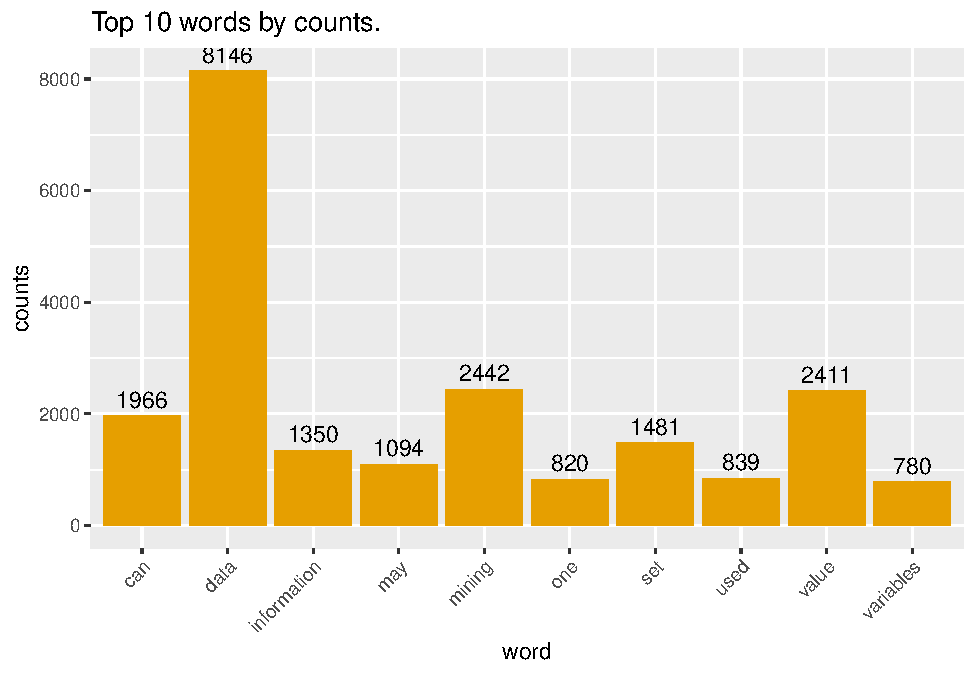
\includegraphics{C:/Users/SUMANP~1/Desktop/RFORDA~1/PROJEC~1/MDSPRJ2/reports/33-PRO~1/figure-latex/unnamed-chunk-21-1.pdf}

\begin{Shaded}
\begin{Highlighting}[]
\NormalTok{mat }\OtherTok{\textless{}{-}} \FunctionTok{as.matrix}\NormalTok{(my\_tdm)}
\NormalTok{freq }\OtherTok{\textless{}{-}}\NormalTok{ mat }\SpecialCharTok{\%\textgreater{}\%} \FunctionTok{rowSums}\NormalTok{() }\SpecialCharTok{\%\textgreater{}\%} \FunctionTok{sort}\NormalTok{(}\AttributeTok{decreasing =}\NormalTok{ T)}

\CommentTok{\# plot word cloud}
\FunctionTok{wordcloud}\NormalTok{(}
  \AttributeTok{words =} \FunctionTok{names}\NormalTok{(freq),}
  \AttributeTok{freq =}\NormalTok{ freq,}
  \AttributeTok{min.freq =} \DecValTok{300}\NormalTok{,}
  \AttributeTok{max.words =} \DecValTok{500}\NormalTok{,}
  \AttributeTok{random.order =} \ConstantTok{FALSE}\NormalTok{,}
  \AttributeTok{colors =} \FunctionTok{brewer.pal}\NormalTok{(}\DecValTok{8}\NormalTok{, }\StringTok{"Dark2"}\NormalTok{),}
  
  \AttributeTok{random.color =} \ConstantTok{TRUE}\NormalTok{,}
  \AttributeTok{rot.per =} \FloatTok{0.35}\NormalTok{,}
  \AttributeTok{use.r.layout =} \ConstantTok{FALSE}
\NormalTok{)}
\end{Highlighting}
\end{Shaded}

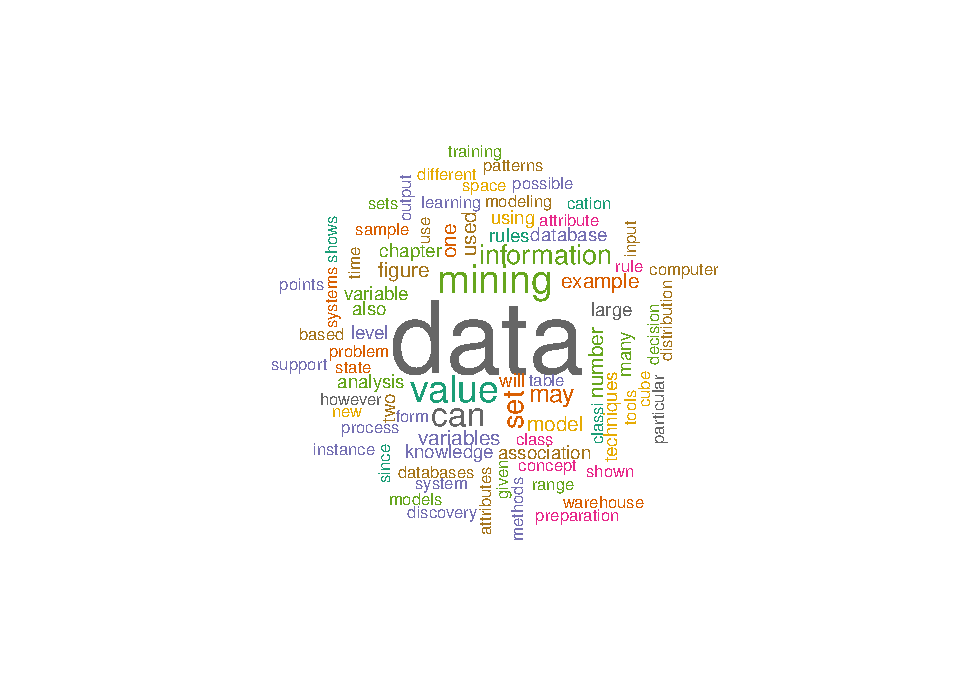
\includegraphics{C:/Users/SUMANP~1/Desktop/RFORDA~1/PROJEC~1/MDSPRJ2/reports/33-PRO~1/figure-latex/unnamed-chunk-22-1.pdf}

\hypertarget{word-correlation}{%
\paragraph{Word Correlation}\label{word-correlation}}

\begin{Shaded}
\begin{Highlighting}[]
\CommentTok{\# correlation between top 600 frequent terms}
\NormalTok{top\_600\_frequent\_tems }\OtherTok{\textless{}{-}} \FunctionTok{findFreqTerms}\NormalTok{(my\_tdm, }\AttributeTok{lowfreq =} \DecValTok{600}\NormalTok{)}
\FunctionTok{plot}\NormalTok{(my\_tdm, }\AttributeTok{terms =}\NormalTok{ top\_600\_frequent\_tems, }\AttributeTok{corThreshold =} \FloatTok{0.2}\NormalTok{, }\AttributeTok{weighting =}\NormalTok{ T)}
\end{Highlighting}
\end{Shaded}

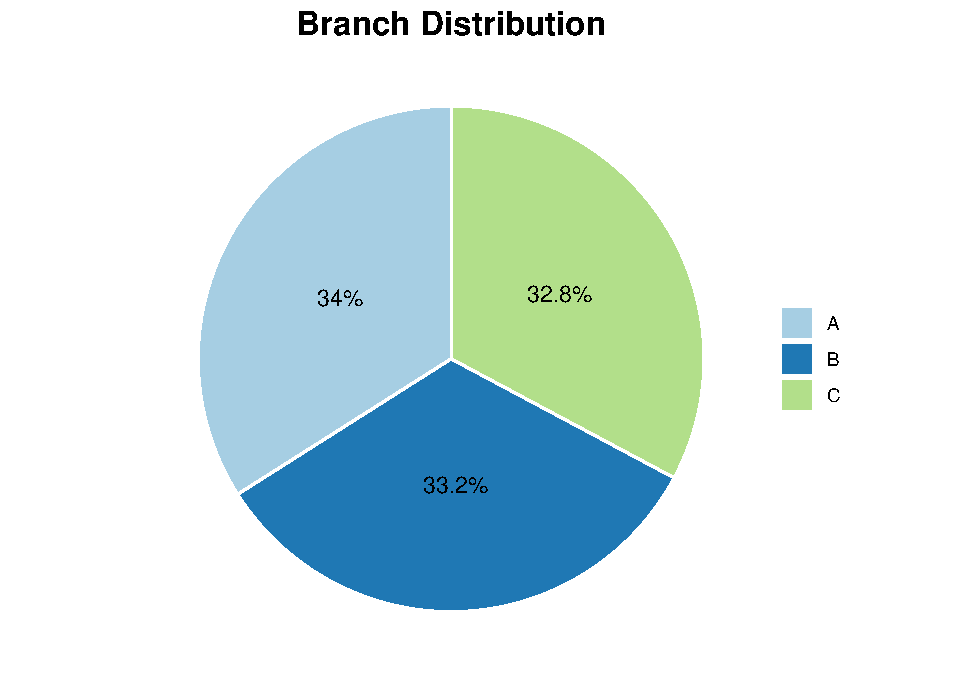
\includegraphics{C:/Users/SUMANP~1/Desktop/RFORDA~1/PROJEC~1/MDSPRJ2/reports/33-PRO~1/figure-latex/unnamed-chunk-23-1.pdf}

\end{document}
